%%%%%%%%%%%%%%%%%%%%%%%%%%%%%%%%%%%%%%%%%%%%%%%%%%%%%%%%%%%%%%%%%%%%%%%%%%%%%%%%
% Limit_Intepretation.tex: Select of showering and tracking events:
%%%%%%%%%%%%%%%%%%%%%%%%%%%%%%%%%%%%%%%%%%%%%%%%%%%%%%%%%%%%%%%%%%%%%%%%%%%%%%%%
\chapter{Limit and Interpretation}
\label{Limit_Results_and_Intepretation_Chapter}
%%%%%%%%%%%%%%%%%%%%%%%%%%%%%%%%%%%%%%%%%%%%%%%%%%%%%%%%%%%%%%%%%%%%%%%%%%%%%%%%
The GMSB model is the leading model we have used as providing the signal topology in our search for NMLLP. As a result, we provide an interpretation of our above results in the context of GMSB.
In GMSB, the neutralino $\tilde{\chi^{0}_{1}}$ is the NLSP and decays to the gravitino $\tilde{G}$ the LSP~(as a result of R-parity conservation) in association with a very energetic photon $\gamma$. Because of the smallness in mass difference between the  $\tilde{\chi^{0}_{1}}$ and the $\tilde{G}$ as well as the coupling, the $\tilde{\chi^{0}_{1}}$ decay to $\tilde{G}$ is delayed and as a result, the photon emitted can arrive late in the calorimeter crystals.  Measuring the arrival time of the photon on ECAL crystals, we can extract important parameters of  theory of GMSB.

\begin{center}
\centering
\mbox{
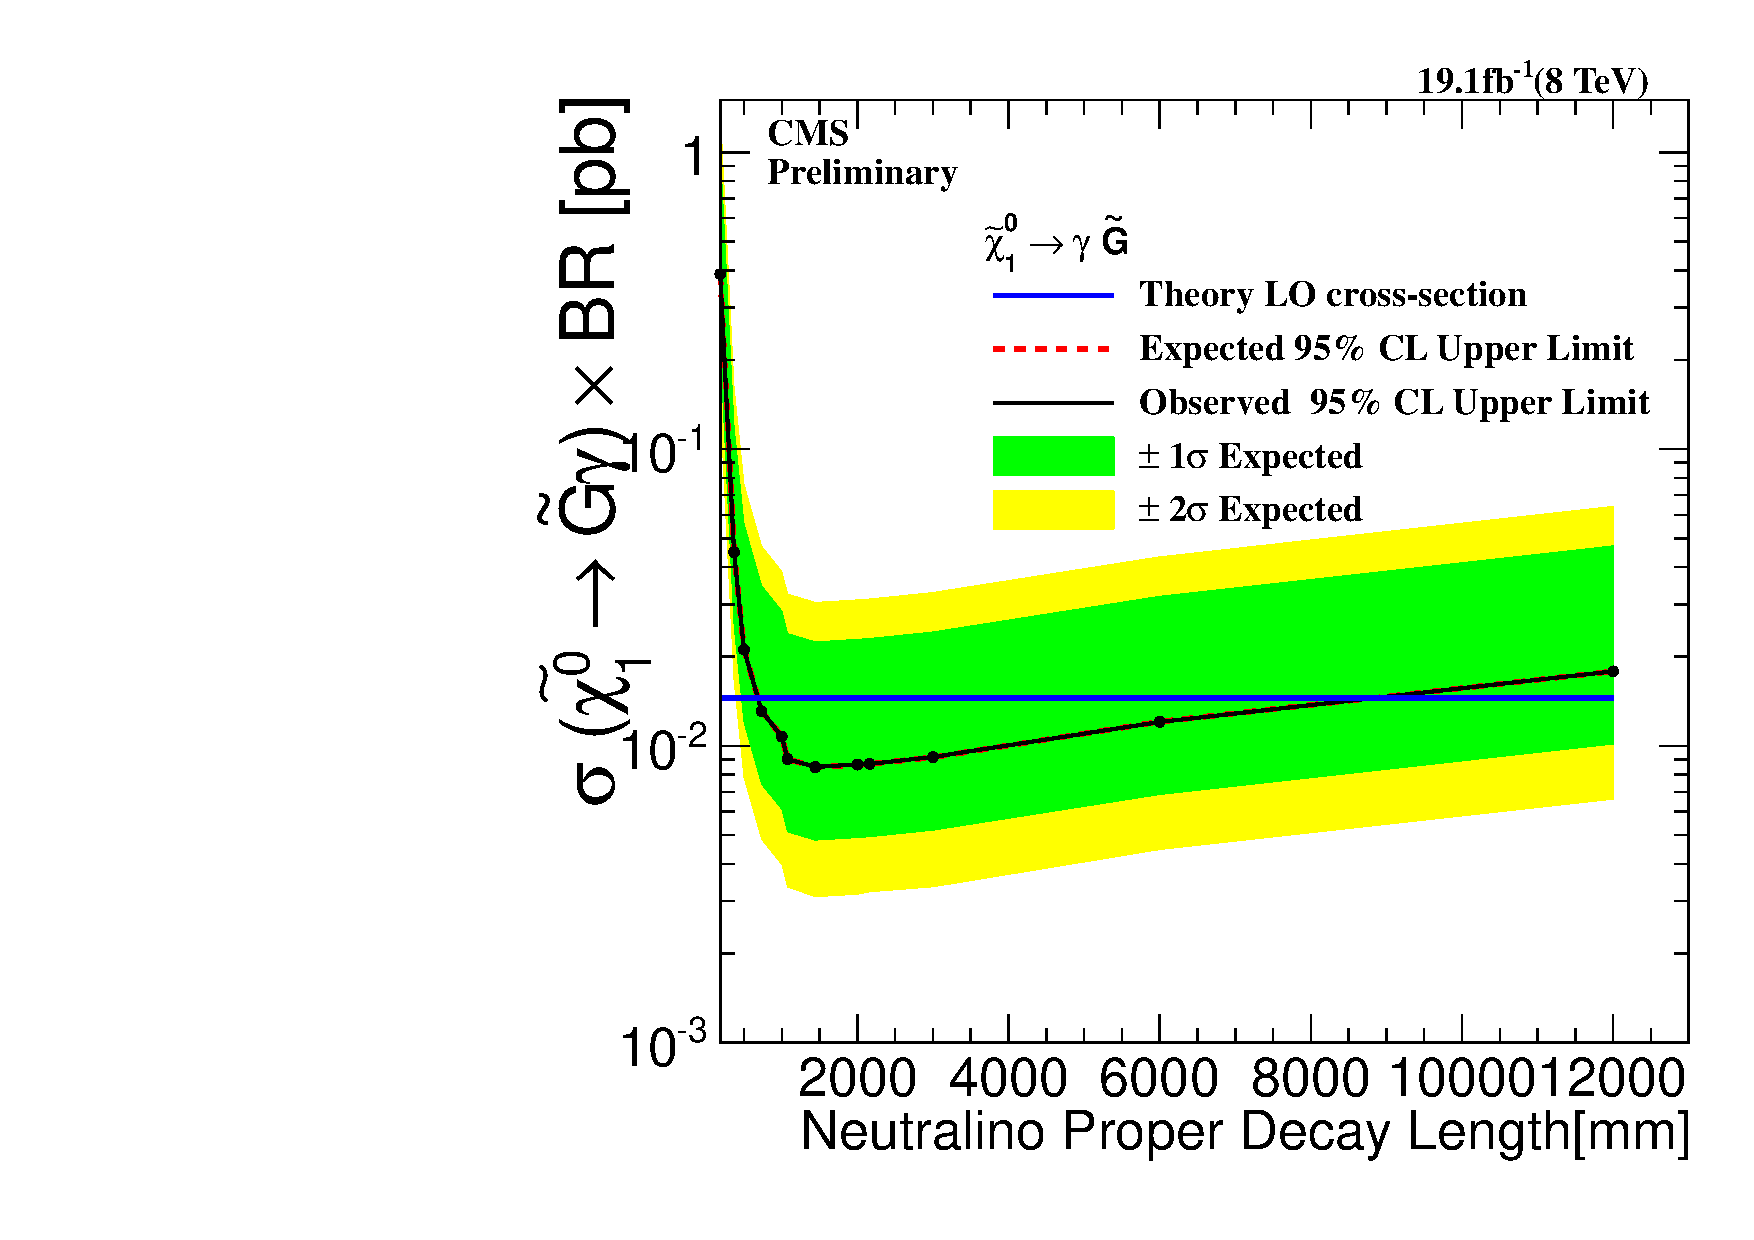
\includegraphics[width=5in]{THESISPLOTS/Neutralino_CrossSecTimesBR_Uplimit.pdf}}
\captionof{figure}{Neutralino production cross section against proper delay length upper limit interpretation in SPS8 model.}
\label{fig:SPS8_Ulimit}
\end{center}


%\begin{figure}[!htb]
\begin{center}
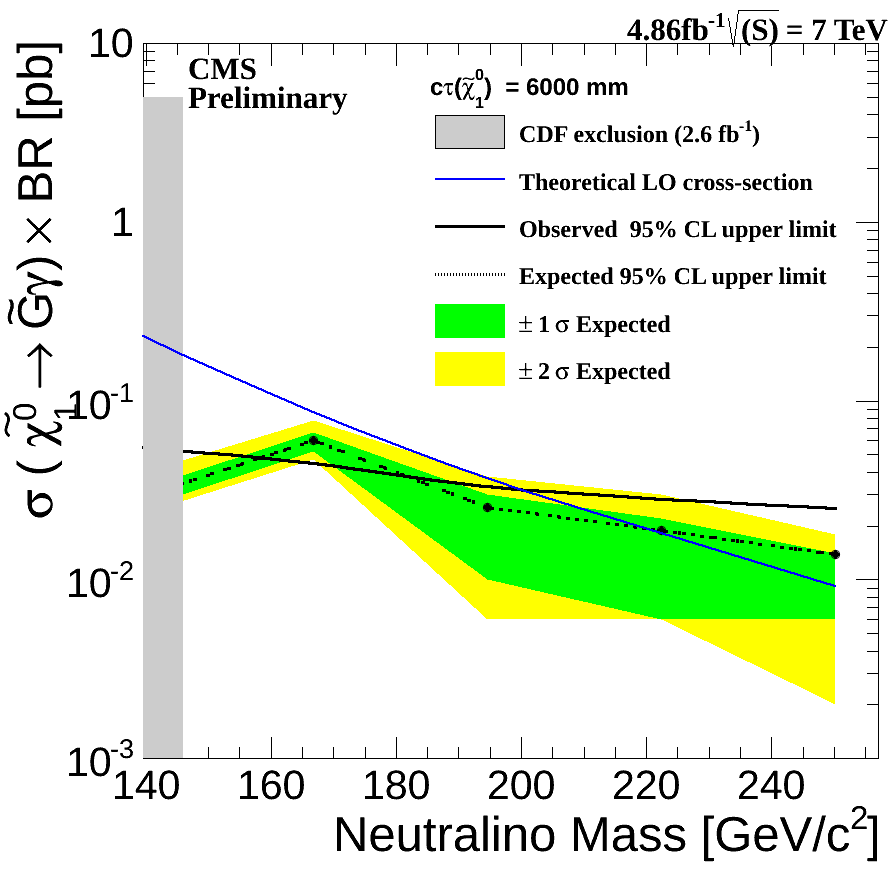
\includegraphics[width=0.49\textwidth,height=0.5\textwidth]{THESISPLOTS/Neutralino_XsecVsMAss_Exclusion_limit_6000.png}
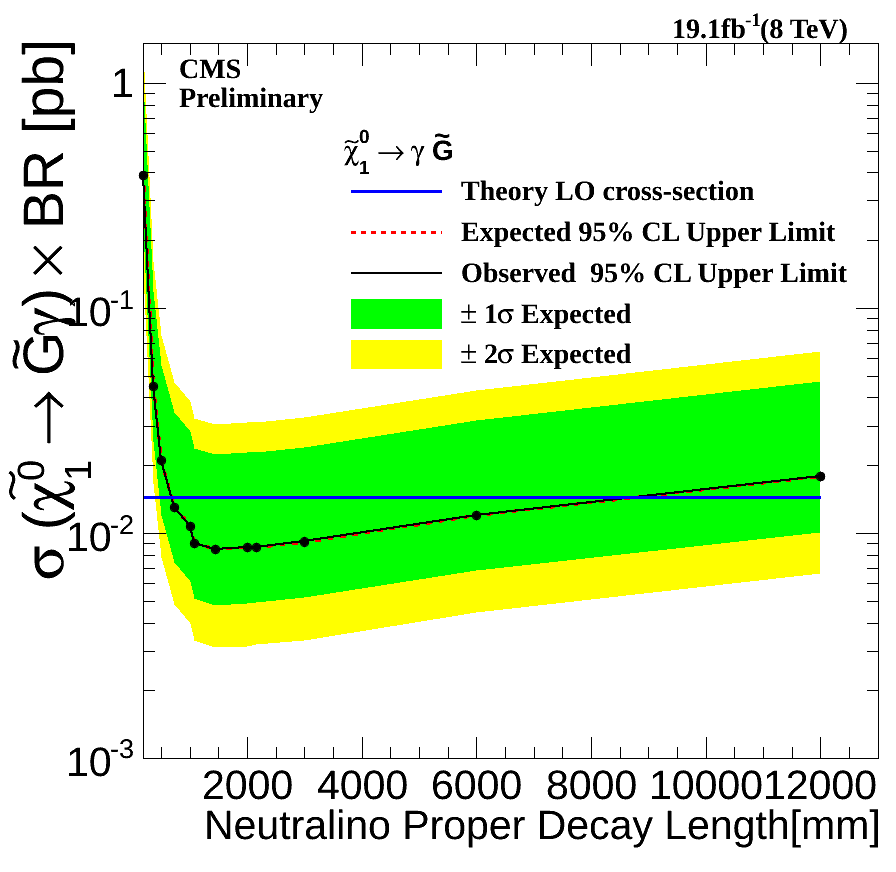
\includegraphics[width=0.49\textwidth,height=0.5\textwidth]{THESISPLOTS/Neutralino_CrossSecTimesBR_Uplimit.png}
\captionof{figure}{Neutralino production cross section against proper delay length upper limit at 95\% confidence levels interpretation in SPS8 model.}
\label{fig:limits}
\end{center}
%\end{figure}


\begin{center}
\centering
\mbox{
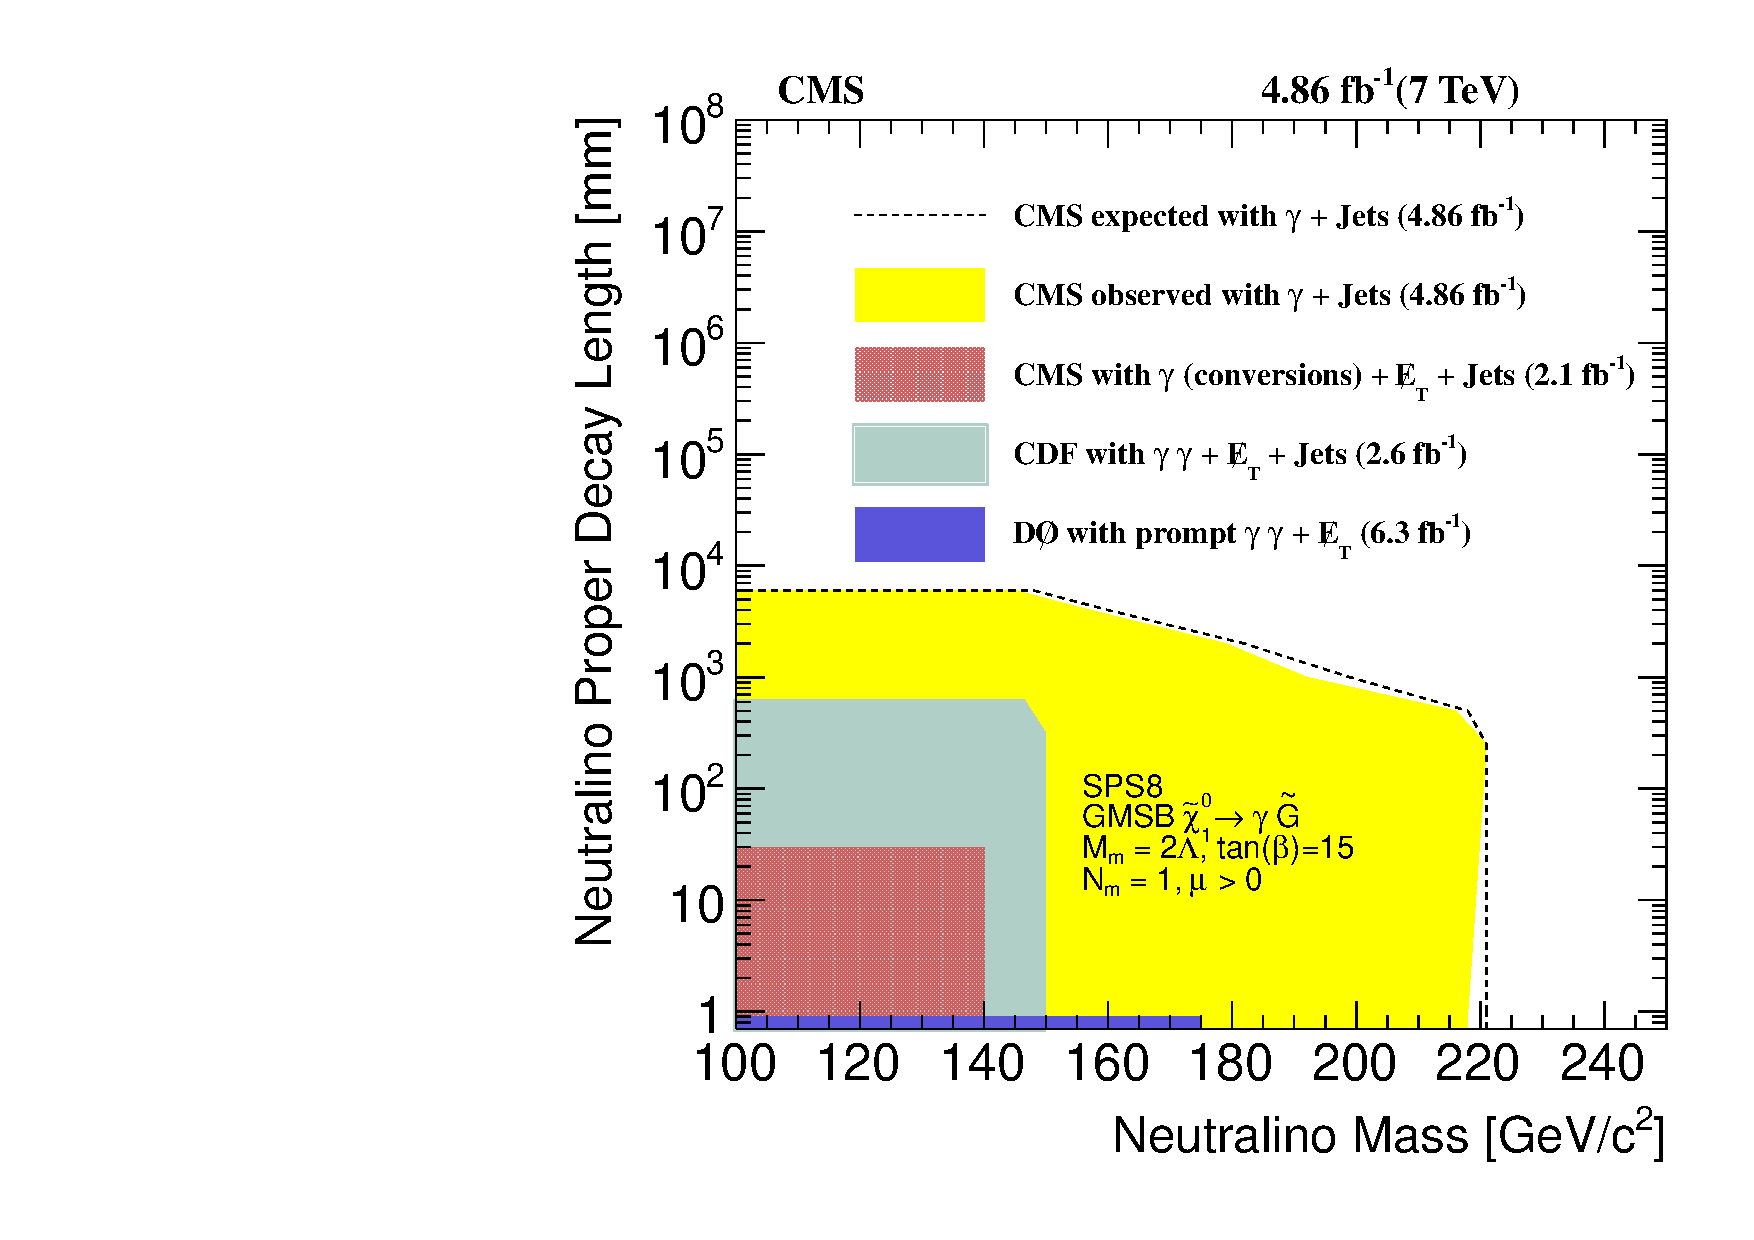
\includegraphics[width=5in]{THESISPLOTS/Neutralino_2D_exclusion.pdf} }
\captionof{figure}{Neutralino two dimensional exclusion limit of neutralino mass ($\Lambda$) against proper delay length upper limit interpretation in SPS8 model in the decay $\tilde{\chi}^{0}_{1} \rightarrow \gamma + \tilde{G}$ with limits from previous experiments shown.}
\label{fig:SPS8_Ulimit}
\end{center}


%%%%%%%%%%%%%%%%%%%%%%%%%%%%%%%%%%%%%%%%%%%%%%%%%%%%%%%%%%%%%%%%%%%%%%%%%%%%%%%%
%%%%%%%%%%%%%%%%%%%%%%%%%%%%%%%%%%%%%%%%%%%%%%%%%%%%%%%
%%%%%%%%%%%%%%%%%%%%%%%%%%%%%%%%%%%%%%%%%%%%%%%%%%%%%%%%%%%%%%%%%%%%%%%%%%%%%%%%
% Possible Future Analysis work!
%%%%%%%%%%%%%%%%%%%%%%%%%%%%%%%%%%%%%%%%%%%%%%%%%%%%%%%%%%%%%%%%%%%%%%%%%%%%%%%%
\section{Future Improvements}
%%%%%%%%%%%%%%%%%%%%%%%%%%%%%%%%%%%%%%%%%%%%%%%%%%%%%%%%%%%%%%%%%%%%

%%%%%%%%%%%%%%%%%%%%%%%%

\subsection{Beam Halo Monitoring Detector}
%\label{Beam Halo Procedure}
%%%%%%%%%%%%%%%%%%%%%%%%%%%%%%%%%%%%%%%%%%%%%%%%%%%%%%%%%%%%%%%%%%%%%%%%%%%%%%%%


%%%%%%%%%%%%%%%%%%%%%%%%%%%%%%%%%%%%%%%%%%%%%%%%%%%%%%%%%%%%%%%%%%%%%%%%%%%%%%%%
\subsection{Back-end Electronics upgrade HCAL}
%\label{hcal)back_end_Electronics}

%%%%%%%%%%%%%%%%%%%%%%%%%%%%%%%%%%%%%%%%%%%%%%%%%%%%%%%%%%%%%%%%%%%%%%%%%%%%%}}}
